%请使用XeLaTeX编译
\documentclass[twocolumn]{ctexart}
\CTEXsetup[format={\Large\bfseries}]{section}%让\section左对齐
\renewcommand{\abstractname}{}%去掉摘要头上的标题
\usepackage[margin=2cm]{geometry}%调整页边距
\usepackage{pifont}%提供圆圈数字输入
\usepackage{graphicx}%插入图片
\usepackage{authblk}%作者、单位
\usepackage{amsmath, bm}%数学公式宏包
\usepackage{esint}%使重积分符号更加紧凑,必须加在amsmath后
\usepackage{amssymb}%特殊数学符号
\usepackage{caption}%图片标题处理
\usepackage{float}%处理图表浮动插入
\usepackage[section]{placeins}%防止图表浮动跨过section
\usepackage{subfigure}%插入多图时用子图显示的宏包
\usepackage{multicol}%调整栏间距
\makeatletter
\def\@cite#1#2{\textsuperscript{[{#1\if@tempswa , #2\fi}]}}
\makeatother%右上角引用文献
\pagestyle{plain}%页码
\setCJKfamilyfont{zhsong}{SimSun}
\setCJKmainfont{SimSun}[BoldFont=FandolSong-Bold]
\renewcommand*{\songti}{\CJKfamily{zhsong}}%定义新宋体命令
\setlength{\belowcaptionskip}{-2pt}
\setlength{\columnsep}{1cm} %调整栏间距为1cm
\begin{document}
	\zihao{5}%设置全文字号为五号
	\everymath{\displaystyle}%设置所有数学公式为displaystyle形式
	\abovedisplayshortskip=5pt%设置数学公式间距
	\belowdisplayshortskip=5pt
	\abovedisplayskip=5pt
	\belowdisplayskip=5pt
	\lineskiplimit=4pt
	\lineskip=4pt
	\title{\vspace{-2cm}{\heiti {\zihao{2}标题}} }%标题
	\date{}%不显示日期
	\author{\kaishu\zihao{-4}作者1 , 作者2 , 作者3\vspace{-1.5em}}%作者名称
	\affil{{{\zihao{6}{\kaishu (单位)}}}\vspace{-6em}}%作者单位
	\ctexset{
		section = {
			format = \heiti\zihao{4}\vspace{-0.6em},
			number = \textbf{\arabic{section}},
		}
	}%设置section格式
	\ctexset{
		subsection = {
			format = \heiti\zihao{5}\vspace{-0.6em},
			number=\textbf{\arabic{section}.\arabic{subsection}},
		}
	}%设置subsection格式
	\twocolumn[
	\begin{@twocolumnfalse}
		\maketitle 
		\begin{abstract}
			\newgeometry{left=1.5cm, right=1.5cm}%调整摘要部分的页边距,与正文对齐
			\noindent{\zihao{-5}{\heiti 摘~~~要 }{\kaishu ~~~这是一段摘要,这是一段摘要,这是一段摘要,这是一段摘要,这是一段摘要,这是一段摘要,这是一段摘要,这是一段摘要,这是一段摘要,这是一段摘要,这是一段摘要,这是一段摘要,这是一段摘要,这是一段摘要,这是一段摘要,这是一段摘要。}}\\
			\noindent{\zihao{-5}\heiti 关键词 }~~~{\zihao{-5}\kaishu 关键词1~~~~关键词2~~~~关键词3}\\
			\\
		\end{abstract}
	\end{@twocolumnfalse}
	]%双栏环境下单栏的摘要
	\section{引言}
	这是一段引言,这是一段引言,这是一段引言,这是一段引言,这是一段引言,这是一段引言,这是一段引言,这是一段引言,这是一段引言,这是一段引言,这是一段引言,这是一段引言,这是一段引言,这是一段引言。\par
	这是一段引言,这是一段引言,这是一段引言,这是一段引言,这是一段引言,这是一段引言,这是一段引言,这是一段引言,这是一段引言,这是一段引言,这是一段引言,这是一段引言,这是一段引言,这是一段引言,这是一段引言,这是一段引言,这是一段引言,这是一段引言,这是一段引言,这是一段引言,这是一段引言。
	
	这是一段引言,这是一段引言,这是一段引言,这是一段引言,这是一段引言,这是一段引言,这是一段引言,这是一段引言,这是一段引言,这是一段引言,这是一段引言,
	这是一段引言,这是一段引言,这是一段引言。
	\section{第二部分}
	\subsection{第一小节}
	这是一个公式
	 \begin{equation}
	 	U\left(\omega,T\right)d\omega =\frac{V}{{\pi}^2c^3}\hbar{\omega}^3e^{-\frac{\hbar\omega}{kT}}d\omega
	\end{equation}
	\subsection{第二小节}
	这是一个图片
	\begin{figure}[H]
		\centering
		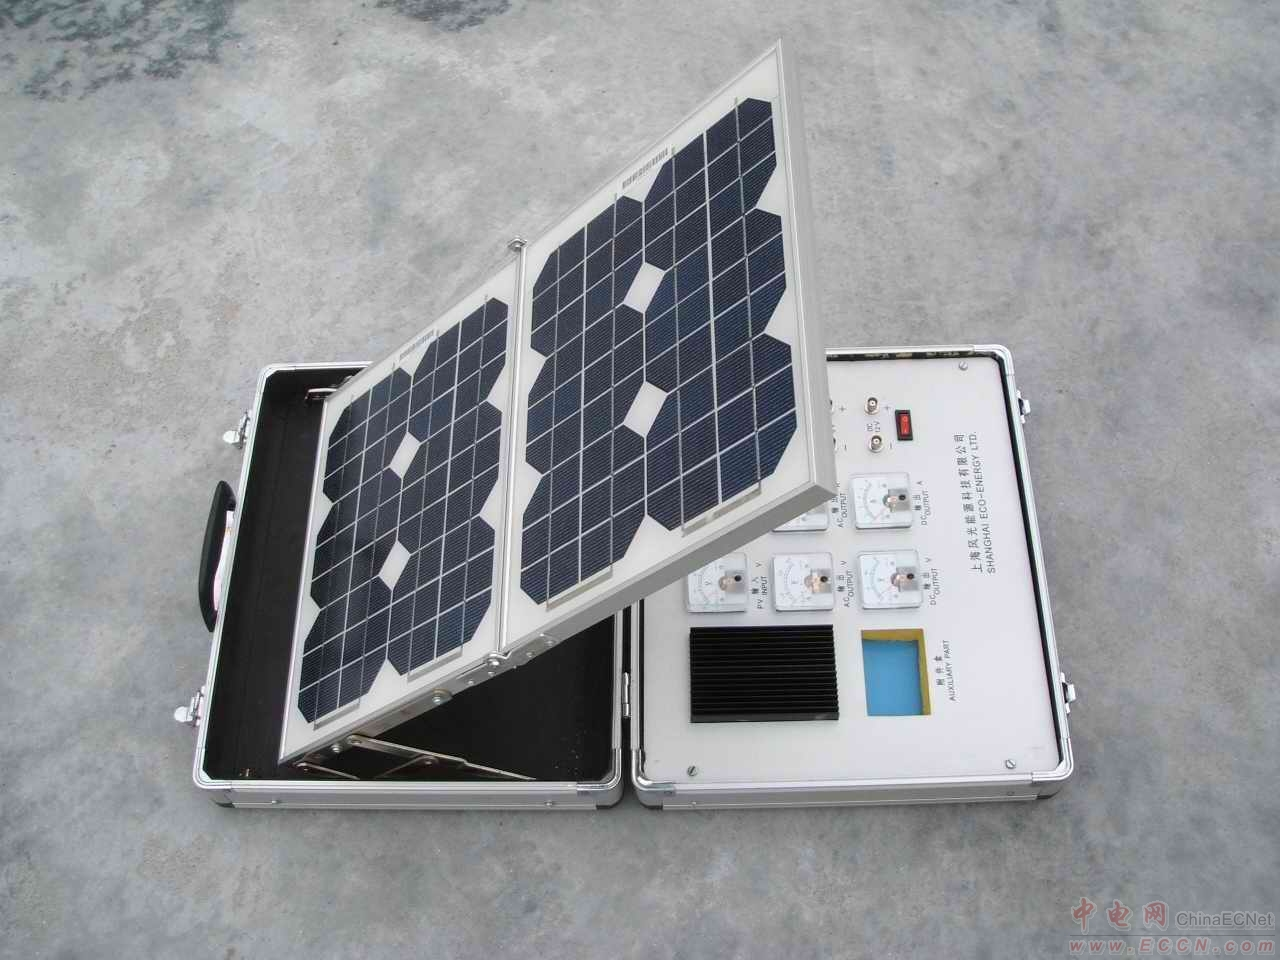
\includegraphics[width=0.3\textwidth]{图片.jpg}
		\caption{这是一个图片}
		\label{fig:example}
	\end{figure}
	\section{第三部分}
	这是一个表格\par
	\begin{tabular}{|c|c|c|}
		\hline
		Header 1 & Header 2 & Header 3 \\
		\hline
		Cell 1 & Cell 2 & Cell 3 \\
		\hline
		Cell 4 & Cell 5 & Cell 6 \\
		\hline
	\end{tabular}
	\subsection{第三小节}
	文献引用1\cite{einstein_uber_1905},文献引用2\cite{hertz_ueber_1887},文献引用3\cite{rayleigh_liii_1900},文献引用4\cite{wien_xxx_1897}
\bibliographystyle{unsrt}
\bibliography{ref}%为参考文献,左侧括号内为bibtex文件名,会按在文章中引用顺序排序。
\end{document}